\documentclass[%
 reprint,
%superscriptaddress,
%groupedaddress,
%unsortedaddress,
%runinaddress,
%frontmatterverbose, 
%preprint,
%preprintnumbers,
%nofootinbib,
%nobibnotes,
%bibnotes,
 amsmath,amssymb,
 aps,
%pra,
%prb,
%rmp,
%prstab,
%prstper,
%floatfix,
]{revtex4-2}

\usepackage{graphicx}% Include figure files
\usepackage{dcolumn}% Align table columns on decimal point
\usepackage{bm}% bold math
\usepackage{physics}
%\usepackage{hyperref}% add hypertext capabilities
%\usepackage[mathlines]{lineno}% Enable numbering of text and display math
%\linenumbers\relax % Commence numbering lines

%\usepackage[showframe,%Uncomment any one of the following lines to test 
%%scale=0.7, marginratio={1:1, 2:3}, ignoreall,% default settings
%%text={7in,10in},centering,
%%margin=1.5in,
%%total={6.5in,8.75in}, top=1.2in, left=0.9in, includefoot,
%%height=10in,a5paper,hmargin={3cm,0.8in},
%]{geometry}

\begin{document}

\preprint{APS/123-QED}

\title{Demonstration of Dory-Guest-Harris Instability Using\\ Magnetostatic Particle-in-Cell Model}% Force line breaks with \\

\author{Evan Bluhm}
%  \altaffiliation[Also at ]{Physics Department, XYZ University.}%Lines break automatically or can be forced with \\
% \author{Second Author}%
%  \email{Second.Author@institution.edu}
% \affiliation{%
%  Authors' institution and/or address\\
%  This line break forced with \textbackslash\textbackslash
% }%

% \collaboration{MUSO Collaboration}%\noaffiliation

% \author{Charlie Author}
%  \homepage{http://www.Second.institution.edu/~Charlie.Author}
% \affiliation{
%  Second institution and/or address\\
%  This line break forced% with \\
% }%
% \affiliation{
%  Third institution, the second for Charlie Author
% }%
% \author{Delta Author}
% \affiliation{%
%  Authors' institution and/or address\\
%  This line break forced with \textbackslash\textbackslash
% }%

% \collaboration{CLEO Collaboration}%\noaffiliation

\date{May 5, 2021}% It is always \today, today,
             %  but any date may be explicitly specified
\begin{abstract}

An existing 1-dimensional electrostatic particle-in-cell code is extended to accommodate a uniform, static external magnetic field. The code is used to simulate the time evolution of a cold ring distribution, resulting in electrostatic waves perpendicular to the magnetic field. These waves are shown to have the same frequency and growth rate as those predicted by linear analysis of the Vlasov equation.

% % \begin{description}
% % \item[Usage]
% % Secondary publications and information retrieval purposes.
% % \item[Structure]
% % You may use the \texttt{description} environment to structure your abstract;
% % use the optional argument of the \verb+\item+ command to give the category of each item. 
% % \end{description}
\end{abstract}

%\keywords{Suggested keywords}%Use showkeys class option if keyword
                              %display desired
\maketitle

%\tableofcontents


\section{Introduction}

Starting from a 1-dimensional electrostatic particle-in-cell code, following the method outlined in \cite{BirdsallCharlesK1991Ppvc}, we extend the model to include a uniform, static external magnetic field. Since the effect of a static, uniform magnetic field is a rotation in velocity space, we must now track two components of the particle's velocity in time. The implementation details of the new magnetic force term are laid out in section II.

Starting with a very basic test of the new functionality, we simulate the motion of a single particle and observe its cyclotron motion, comparing the frequency to that determined by the field strength. As a more serious benchmark of the model, we simulate the time evolution of a cold ring distribution. As described in \cite{PhysRevLett.14.131}, the cold ring distribution is conditionally stable, with unstable modes possible for certain simulation parameters. We observe these unstable modes using our code, and compare the growth rates and oscillation frequencies to those predicted by linear theory.

\section{Magnetostatic 1D2V Particle-in-Cell}

Starting from an electrostatic particle-in-cell (PIC) model which evolves only position $x$ and velocity $v_x$ along a single dimension (1D1V), we incorporate the effect of a uniform, static magnetic field $\vec B_0$. The magnetic field is assumed to be perpendicular to the particle motion, so without loss of generality $\vec B_0 = B_0 \vu z$. We must now include in our model the velocity of each particle in the $y$-direction, bringing the number of dimensions to track for each particle up to three (1D2V). The equation of motion is now the standard Lorentz force in position $\vec x$ and velocity $\vec v$:
\begin{equation}
m \dv{\vec v}{t} = q (\vec E + \vec v \cross \vec B) \qquad \dv{\vec x}{t} = \vec v
\end{equation}
Recalling that our leapfrog integrator is centered in time with velocity at the half-integer time steps, we require a finite difference scheme to advance $\vec v(t - \Delta t / 2)$ to $\vec v(t + \Delta t / 2)$. The $\vec v \cross \vec B$ term is simply a rotation in the $x-y$ plane, but since translation and rotation do not commute, rotating either before or after applying the acceleration due to the electric field will break the time centering of our leapfrog scheme. Instead, we perform a Strang splitting of the particle push, breaking the velocity advance into three finite differences \cite{BirdsallCharlesK1991Ppvc}:
\begin{enumerate}
    \item First, a half-acceleration using the electric field calculated from Poisson's equation at time $t$. Since there is no electric field in the $y$-direction, $v_y$ does not accelerate.
    \begin{eqnarray}
    v_x(t') & = & v_x \left( t - \frac{\Delta t}{2} \right) + \frac{q}{m} E_x(t) \frac{\Delta t}{2} \\
    v_y(t') & = & v_y \left( t - \frac{\Delta t}{2} \right)
    \end{eqnarray}
    \item Rotate $\vec v$ in the $x-y$ plane by angle $\theta = - \omega_c \Delta t$, where $\omega_c$ is the cyclotron frequency $q B_0 / m$:
    \begin{equation}
    \begin{bmatrix}
    v_x(t'') \\ v_y(t'') 
    \end{bmatrix} = \begin{bmatrix}
    \cos \omega_c \Delta t & \sin \omega_c \Delta t \\ - \sin \omega_c \Delta t & \cos \omega_c \Delta t
    \end{bmatrix} \begin{bmatrix}
    v_x(t') \\ v_y(t')
    \end{bmatrix}
    \end{equation}
    \item Finally, complete the time-centered acceleration:
    \begin{eqnarray}
    v_x \left( t + \frac{\Delta t}{2} \right) & = & v_x(t'') + \frac{q}{m} E_x(t) \frac{\Delta t}{2} \\
    v_y \left( t + \frac{\Delta t}{2} \right) & = & v_y(t'')
    \end{eqnarray}
\end{enumerate}
Strang splitting is both centered in time, and second-order accurate in time, allowing us to retain the second-order accuracy and conservation properties of our leapfrog integrator.

\begin{figure}
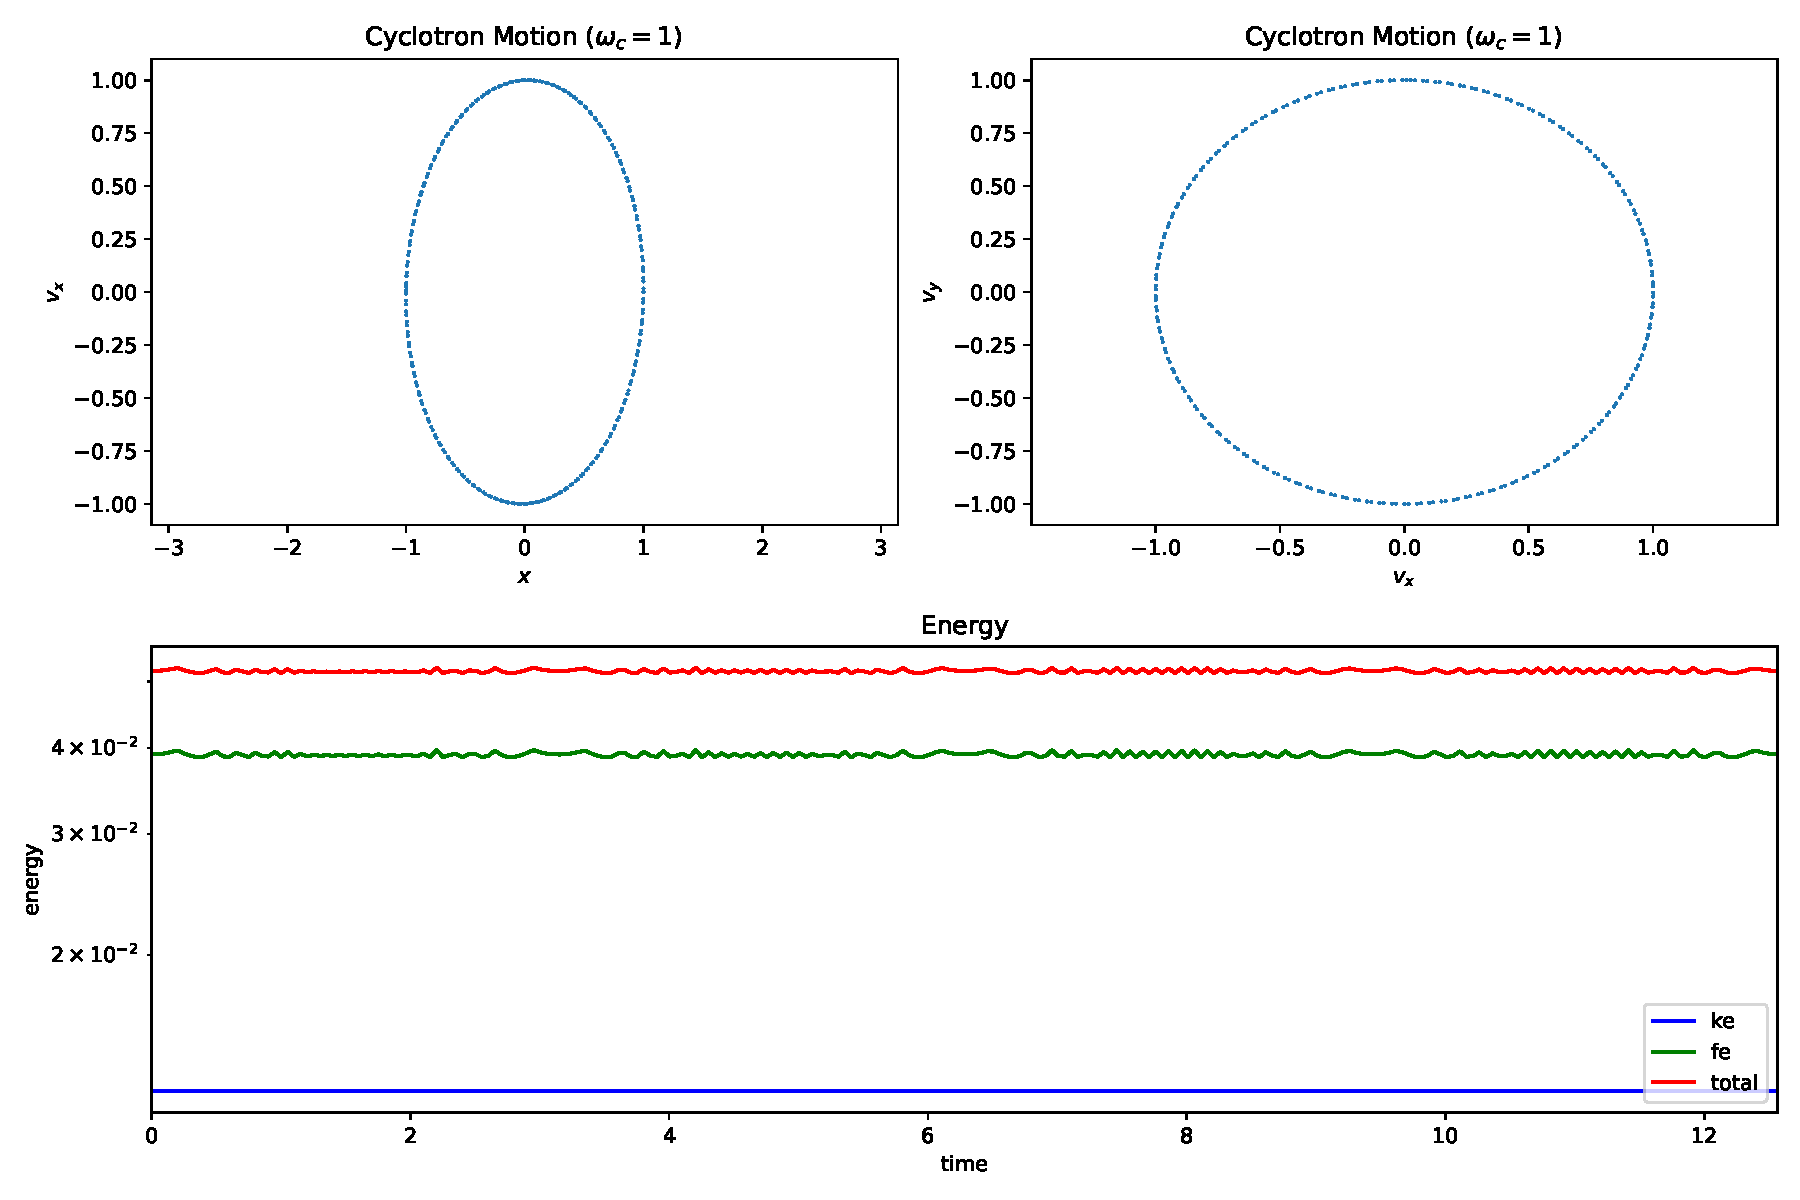
\includegraphics[width=0.9\linewidth]{proj4/traces_1_particles.pdf}
\caption{\label{fig:cyclotron-motion-demo}Traces of a single particle released at $t=0$ with $(x, v_x, v_y) = (-1, 0, 1)$. The static magnetic field $B_0$ has been set such that $\omega_c = 1$. The particle travels in cyclotron motion indefinitely, oscillating in both $x$ and $v_x$ with frequency $\omega = \omega_c$. In the upper-left, the particle is shown oscillating at $\omega_c$ in $x$ and $v_x$, and in the upper-right the same oscillation is observed in $v_x$ and $v_y$. Below, the total energy, total kinetic energy, and total electric field energy are plotted. Since the external magnetic field does not alter the energy of the particle, all three are constant.}
\end{figure}

\section{Dory-Guest-Harris Instability: Linear Analysis}

% To determine the behavior of plasma waves in our magnetostatic model, we begin by linearizing the Vlasov equation
% \begin{equation}
% \pdv{f}{t} + ( \vec v \cdot \grad)f + \frac{q}{m}(\vec E + \vec v \cross \vec B) \cdot \grad _v f = 0
% \end{equation}
To search for waves which propagate perpendicular to the external magnetic field $\vec B = B_0 \vu z$, we express the distribution function $f(x, v_x, v_y, t)$ as the sum of a static equilibrium distribution $f_0(x, v_\perp)$ and a small, plane wave perturbation of the form $f_1 = \hat{f}_1 e^{i(\vec k \cdot \vec x - \omega t)}$, where $v_\perp$ is the velocity in the plane perpendicular to $\vec B$, and $\vec k$ has no component parallel to $\vec B$. We assume a similar perturbation of the electric field $\vec E_1 = \hat E_1 e^{i ( \vec k \cdot \vec x - \omega t)}$. Assuming the magnitude of the perturbation is small and discarding second-order terms, the linearized Vlasov equation and Gauss's law read:
\begin{equation}
\pdv{f_1}{t} + \vec v \cdot \pdv{f_1}{\vec x} + \frac{Z}{M} \left( \vec E_1 \cdot \pdv{f_0}{\vec v} + \frac{\omega_c}{\omega_p} \vec v \cross \vu z \cdot \pdv{f_1}{\vec v} \right)
\end{equation}
\begin{equation}
\div \vec E_1 = Z \int f_1 \dd \vec v
\end{equation}
where $M$ is the ratio of the particle's mass to the electron mass, $Z$ is the ratio of the particle's charge to the electron charge, $\omega_p$ is the electron plasma frequency, and $\omega_c = e B / m_e$ is the cyclotron frequency.

Dory, Guest, and Harris \cite{PhysRevLett.14.131} showed that for ring velocity distributions of the form
\begin{equation}
f_0(v _\perp) = \frac{1}{2 \pi v_\perp} \delta(v ^2 - v_\perp ^2) \label{eqn:ringdist}
\end{equation}
there exist unstable solutions for certain values of $\omega_p ^2 / \omega_c ^2$ and $k v_\perp / \omega_c$. The closed form of the dispersion relation $D(k, \omega) = 0$ for this equilibrium distribution is derived in detail in Ref. \cite{VogmanG.V2014Diaa}:
\begin{equation}
0 = 1 + M \frac{\omega_p ^2}{\omega_c ^2} \int _0 ^\pi \frac{\sin (\omega \tau / \Omega_C)}{\sin ( \omega \pi / \Omega_c)} \sin(\tau) F_0(\tau + \pi) \dd \tau \label{eqn-dispersion}
\end{equation}
where $\Omega \equiv Z \omega_c / M \omega_p$ is the reduced frequency and $J_0$ is the zeroth Bessel function of the first kind, and $F_0(\tau)$ is given by:
\begin{equation}
F_0(\tau) = \int _0 ^\infty f_0 ( v_\perp) J_0 \left( 2 \frac{k_\perp v_\perp}{\Omega_c} \sin \frac{\tau}{2} \right) 2 \pi v_\perp \dd v_\perp 
\end{equation}
For a particular value of $\omega_p$, the dispersion relation gives solutions $\omega$ which may be real, imaginary, or complex, depending on the value of $k v_\perp / \omega_c$. The solutions for $\omega_p ^2 / \omega_c ^2 = 10$ are displayed in Figure \ref{fig:dgh-dispersion}.

\begin{figure}
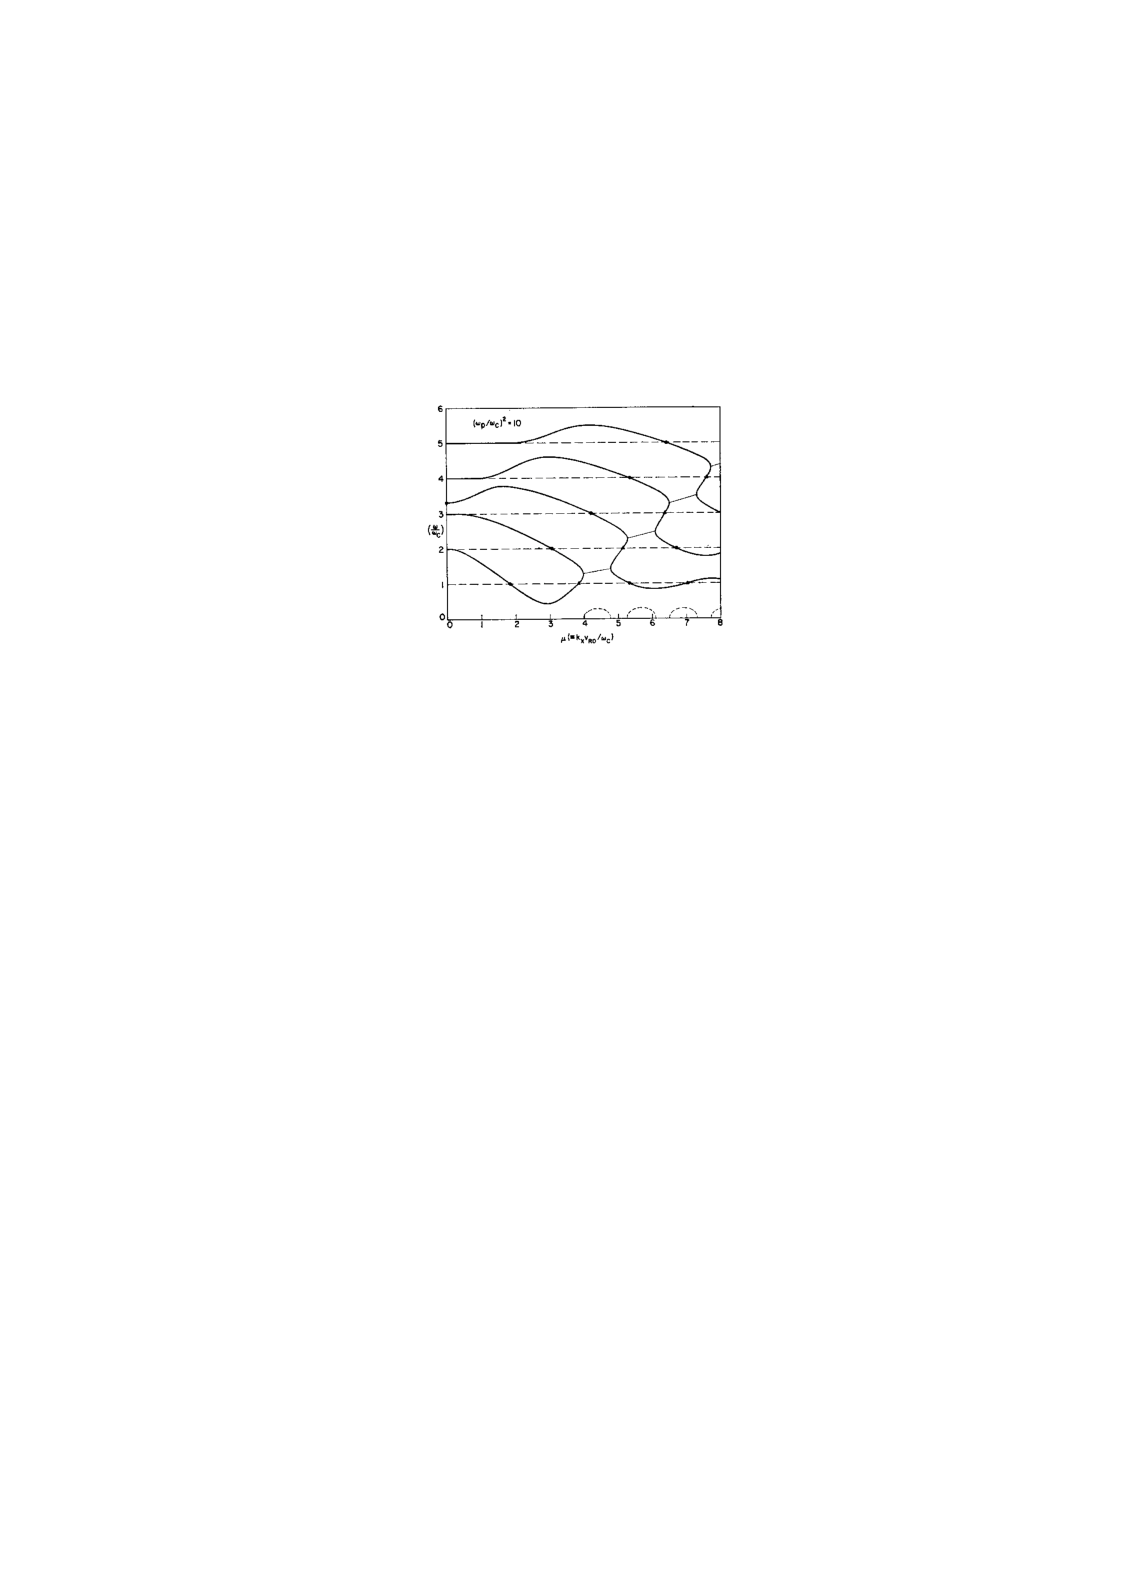
\includegraphics[width=\linewidth]{proj4/dispersion-dgh.pdf}
\caption{\label{fig:dgh-dispersion}Dispersion diagram for the Dory-Guest-Harris instability for a cold ring equilibrium distribution, as given in Ref. \cite{CrawfordF.W1965AIoP}. The solutions $\omega$ for $(\omega_p / \omega _c)^2= 10$ are conditionally stable, depending on the parameter $\mu \equiv k v_\perp / \omega_c$. Solid lines represent real values of $\omega$. Dashed lines represent imaginary components of complex-valued solutions, and the short straight interconnecting lines are their real components. The ring distribution has only stable (oscillatory) solutions for $\mu < 4$. At larger values of $\mu$ there are a series of harmonic modes with complex-valued frequency, which will both oscillate and grow/decay exponentially in time.}
\end{figure}

\section{Dory-Guest-Harris Instability: PIC Model}

To demonstrate the Dory-Guest-Harris instability within our magnetostatic PIC model, we must supply an initial ensemble of particles and velocities which approximates the distribution given in Eqn. \ref{eqn:ringdist}, with an initial perturbation of the form $f_1 = \hat f_1 e^{i (k x - \omega t)}$. We first select a series of $N_x$ uniformly spaced positions $x_0$ distributed across the periodic domain $(-\pi, \pi)$. Then, we apply a small perturbation to these initial positions:
\begin{equation}
x'_0 = x_0 + \delta \cos(k x_0)
\end{equation}
where $\delta$ is the size of the initial perturbation and $k$ is the wavenumber of the solution mode we wish to excite. At each position $(x'_0)_i$, we then fill the velocity space $(v_x, v_y)$ with a sequence of $N_v$ values at equally spaced angles $\theta$, such that
\begin{equation}
\theta_{n_v} = \frac{2 \pi n_v}{N_v} \qquad n_v = 0, 1, \ldots N_v - 1 
\end{equation}
\begin{equation}
(v_x)_i = v_\perp \cos (\theta_{n_v}) \quad (v_y)_i = v_\perp \sin (\theta_{n_v})
\end{equation}

In the limit $N_v \rightarrow \infty$ and $N_x \rightarrow \infty$, this initial distribution becomes $f_0(v_\perp) + f_1(x, t=0)$. The initial distribution and the resulting initial density perturbation are shown in Figure \ref{fig:dgh-initial-distribution}. The function \texttt{set\_initial\_conditions()} within the \texttt{run\_dgh.py} module initializes this distribution and runs the PIC simulation for parameterized values of $\omega_p$, $\omega_c$, and $k v_\perp / \omega_c$.

\begin{figure}
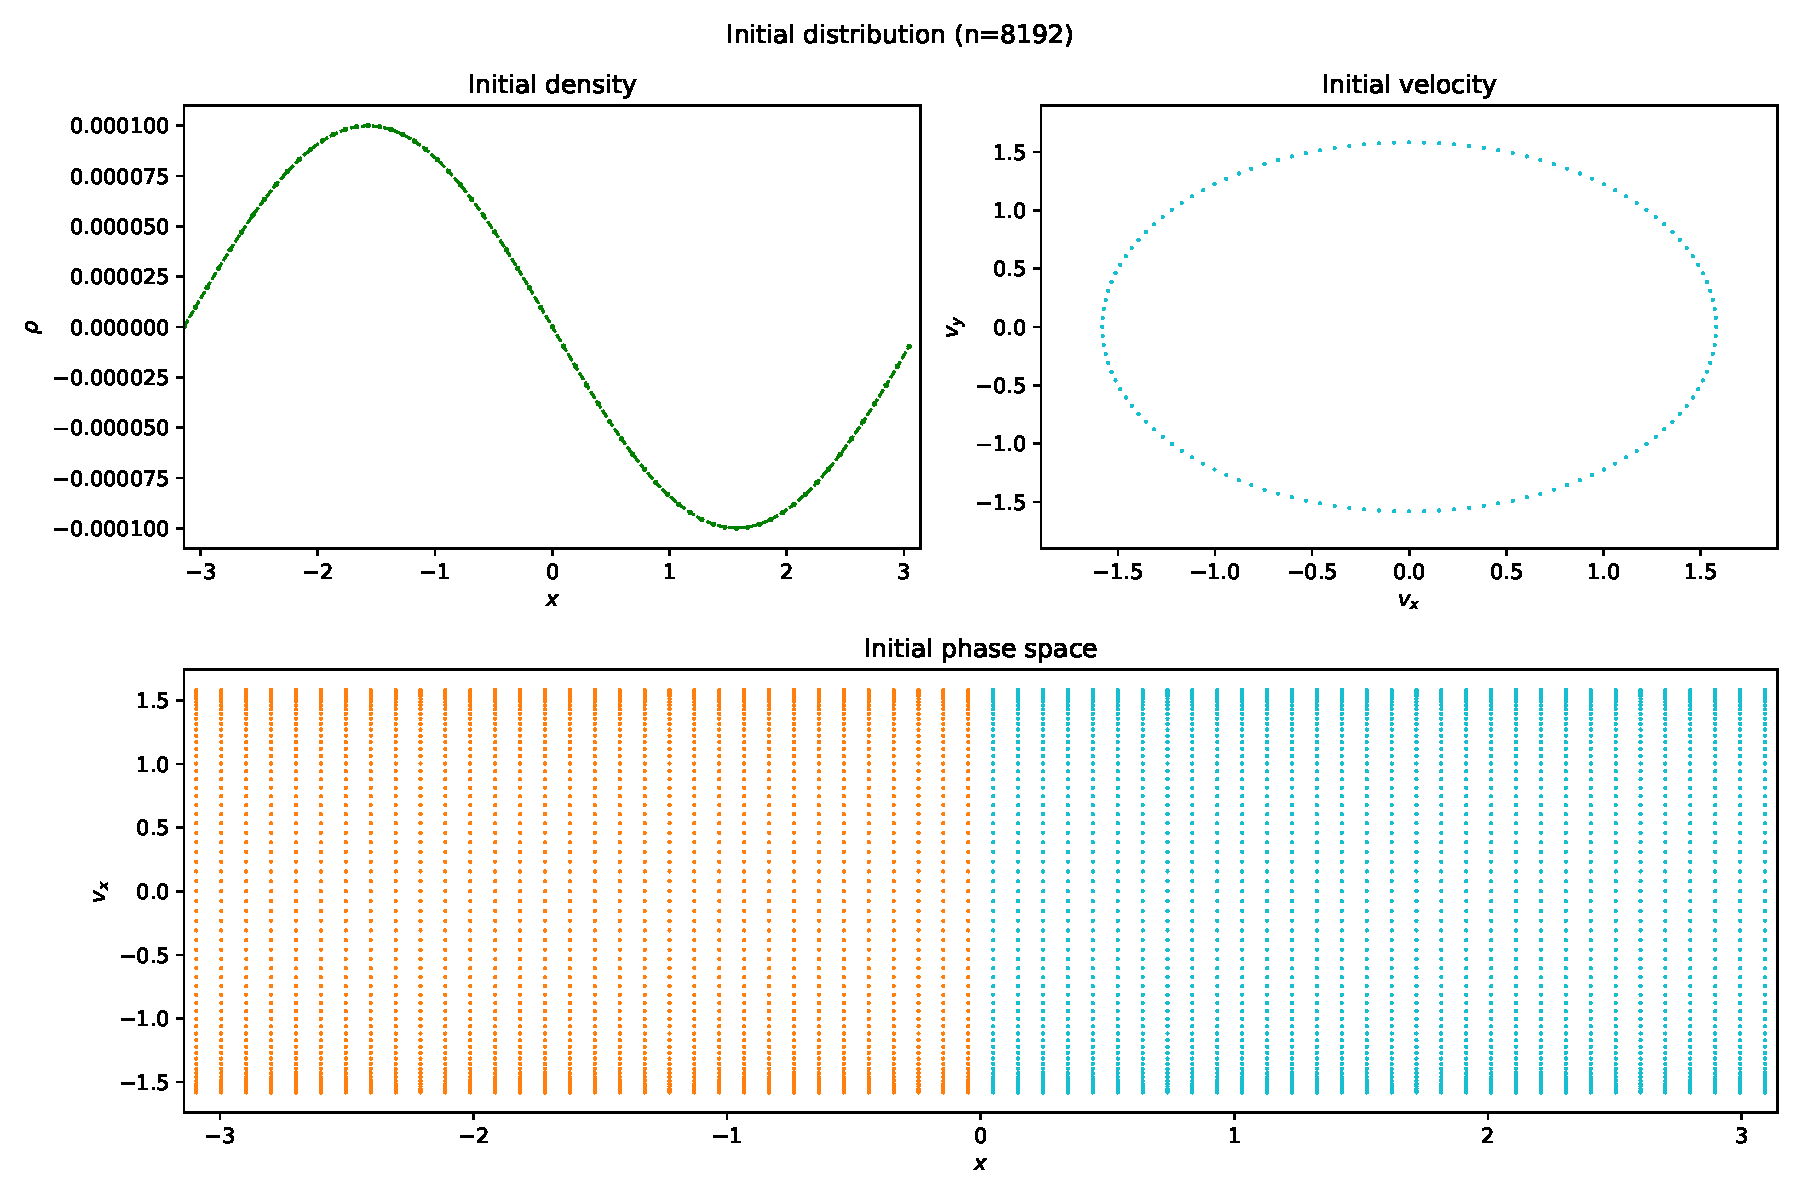
\includegraphics[width=0.9\linewidth]{proj4/initial_hist_8192_particles.pdf}
\caption{\label{fig:dgh-initial-distribution}Initial state of $N = 8192$ particles, approximating the cold ring distribution of Eqn. \ref{eqn:ringdist}. The parameters for particle spacing, grid spacing, and initial perturbation are $N_v = 128$, $N_x = 64$, $M = 64$, $\delta = 10^{-4}$.}
\end{figure}

\section{Results}

With $\omega_p = 1$ and $\omega_c = 1/\sqrt{10}$, we ran the PIC code with various values of $\mu \equiv k v_\perp / \omega_c$ in the range $(4.0, 6.6)$. For $4.0 < \mu < 5.7$, we should find a complex-valued solution $\omega$ to the dispersion relation, as shown as the dashed line in Figure \ref{fig:dgh-dispersion}. For a complex valued $\omega$, a positive imaginary part indicates a solution with exponential growth, and a negative imaginary part indicates a solution with exponential decay. Since the complex conjugate of a complex valued solution is also a solution, and exponential growth dominates over the exponential decay, the resulting wave (and the magnitude of the electric field $\vec E$) should have an exponentially increasing amplitude with growth constant $\text{Im}(\omega)$, and oscillate with frequency $\text{Re}(\omega)$.

For $\mu = 4.1$, the growth of the total electric field energy ($\sim \int E^2 \dd x$) is shown in Figure \ref{fig:dory-guest-harris-4.10}. Initially, the electric field is very small since the equilibrium field is zero and the initial perturbation produces a small net density. Over the course of $\sim 10$ cycles of the plasma frequency, a dominant oscillatory mode emerges and grows over many decades. After $~30$ cycles of the plasma frequency, the perturbation has grown to non-linear size, resulting in a rapid collapse of the cold ring distribution to a thermal velocity distribution as shown in Figure \ref{fig:snapshots-velocity-phase}. We may determine the complex frequency of the excited mode by measuring the frequency of oscillations and the exponential growth rate. Fitting a linear regression to $\ln(U_E)$ over the range of linear growth gives twice the imaginary component of $\omega$, since the field energy is proportional to the square of the electric field. A  count of the number of oscillations over time gives the real part of $\omega$. For $\mu = 4.1$, we observe $\omega / \omega_c = 1.30 + 0.190i$, in good agreement with the complex $\omega$ shown in Figure \ref{fig:dgh-dispersion}.

Performing the same simulation with $\mu = 5.0$, the linear analysis predicts only real values of $\omega$. The perturbation should oscillate at the various harmonic frequencies shown in Figure \ref{fig:dgh-dispersion}, but should not grow over time. The evolution of the field energy $U_E$ over time is shown in Figure \ref{fig:dory-guest-harris-5.0}. As expected, the only motion is oscillatory, and there are no unstable growth modes. A discrete Fourier transform of the field energy over time reveals modes at $\omega = 1.2 \omega_c$, $1.6 \omega_c$, and $2.4 \omega_c$. These are the first few harmonic modes shown in Figure \ref{fig:dgh-dispersion}.

Repeating this process for various values of $\mu$, we observe the complex frequencies reported in Table \ref{tab:frequency-values}. As predicted by the linear theory, the complex solutions to the dispersion relation follow the pattern visualized in Figure \ref{fig:dgh-dispersion}. The imaginary component of each complex solution falls between $0$ and $0.4 \omega_c$, while the real component jumps suddenly by roughly $\omega_c$ between regions of stability.

\begin{figure}
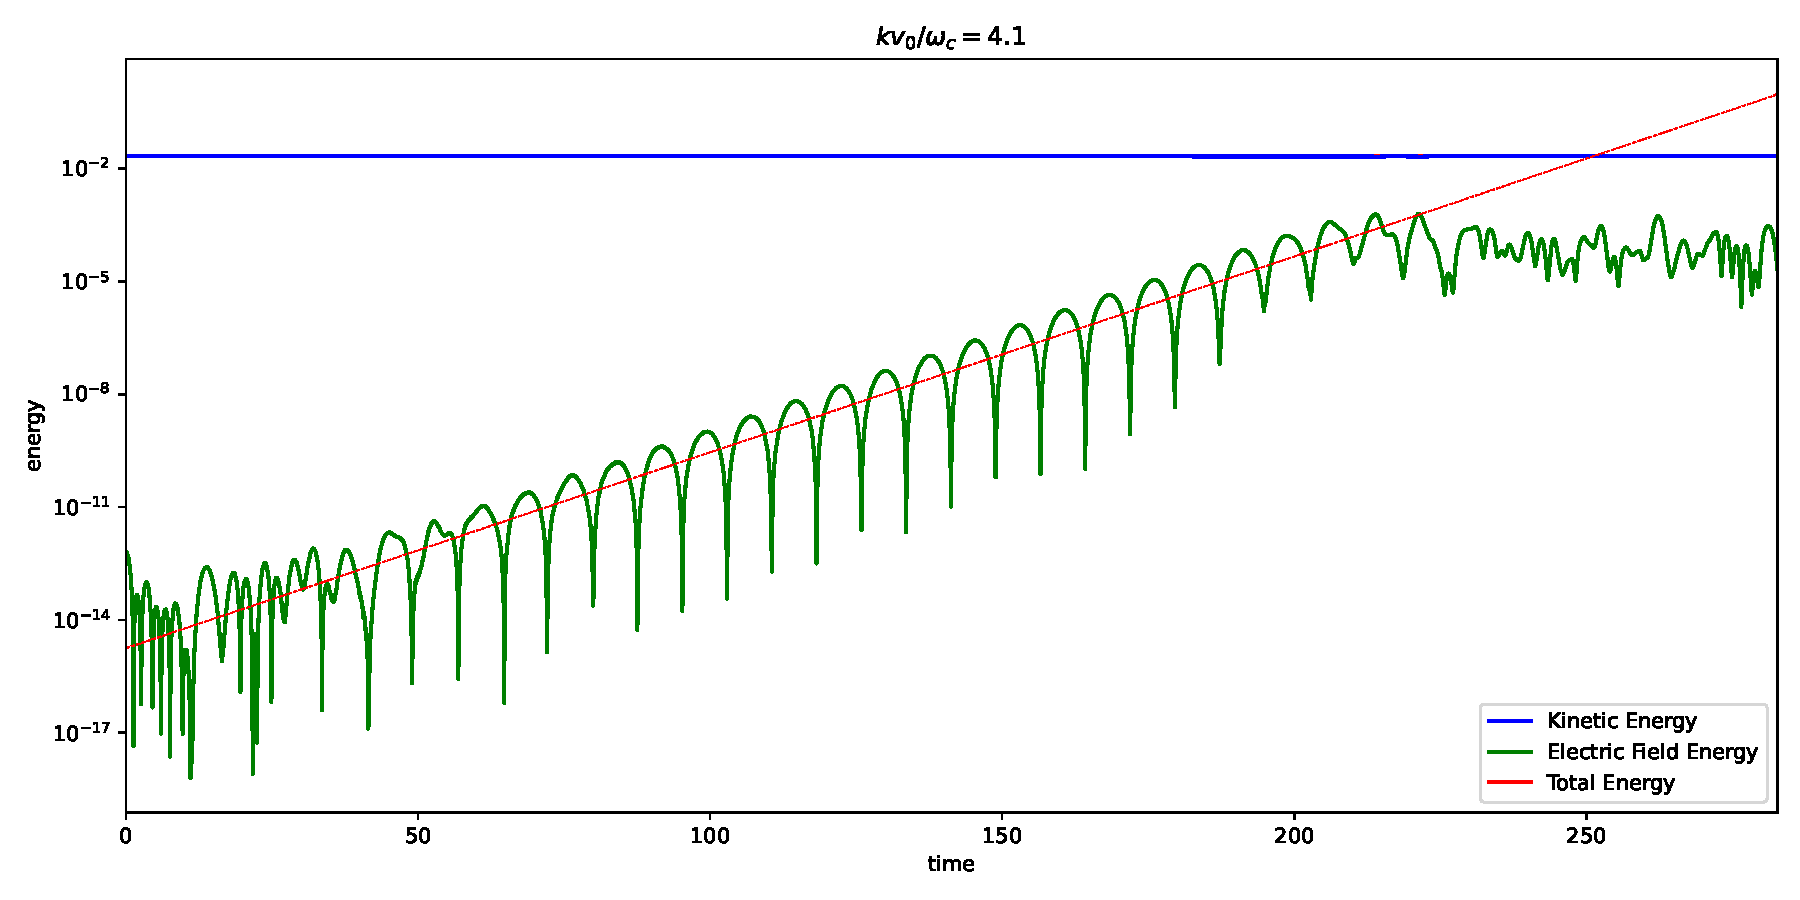
\includegraphics[width=0.9\linewidth]{proj4/dgh_4.10.pdf}
\caption{\label{fig:dory-guest-harris-4.10}Growth and oscillation of the electric field energy over time demonstrates the presence of an excited mode with a complex $\omega$. In this simulation, $\omega_c = 1/\sqrt{10}$, $\omega_p = 1$, $k = 1$ and $v_\perp = 1.42$. Time is normalized by the plasma frequency. The least squares regression fit to the period of linear growth is shown as a red dashed line. The slope of the exponential growth is the complex part of $\omega$, and the oscillation frequency is the real part, giving $\omega / \omega_c = 1.30 + 0.190i$.}
\end{figure}

\begin{figure}
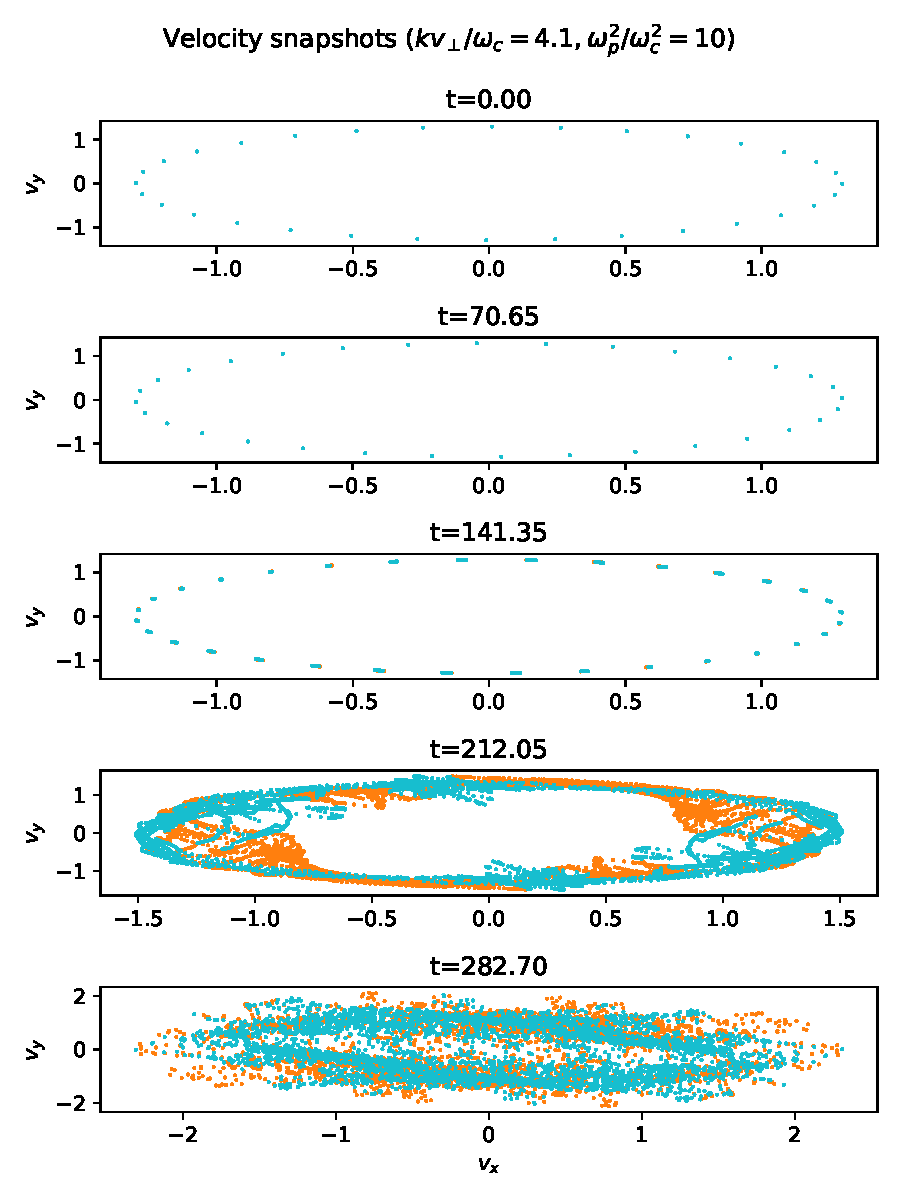
\includegraphics[width=0.9\linewidth]{proj4/snapshots_velocity_phase_space.pdf}
\caption{\label{fig:snapshots-velocity-phase}Rapid collapse of the initial cold ring velocity distribution shown in Figure \ref{fig:dgh-initial-distribution} due to the presence of an unstable mode. The color of each particle is the same as that shown in the initial state in Figure \ref{fig:dgh-initial-distribution}.}
\end{figure}

\begin{figure}
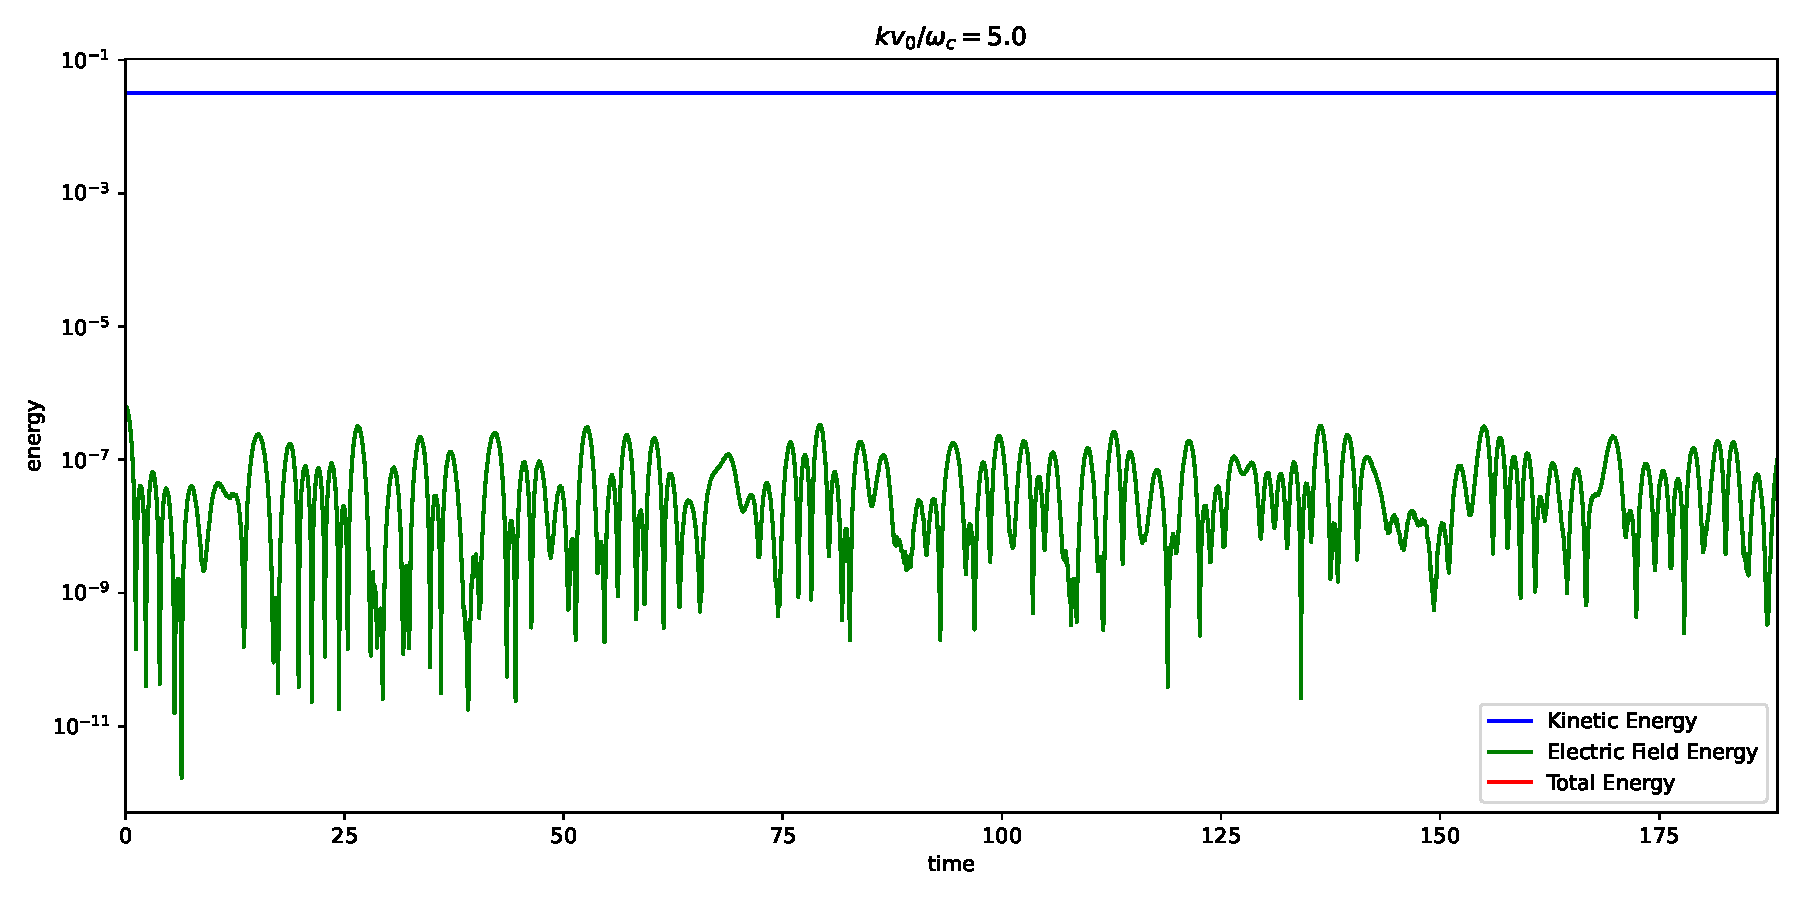
\includegraphics[width=0.9\linewidth]{proj4/dgh_5.0.pdf}
\caption{\label{fig:dory-guest-harris-5.0}Electric field energy over time for $\mu = 5.0$. The field energy oscillates at a combination of harmonic real frequencies given by the roots of Eqn. \ref{eqn-dispersion}. Since there are no complex or imaginary solutions to Eqn. \ref{eqn-dispersion} for $\mu = 5.0$ and $\omega_p ^2 / \omega_c ^2 = 10$, the system is conditionally stable and none of the oscillatory modes grow over time.}
\end{figure}

\begin{figure}[b]
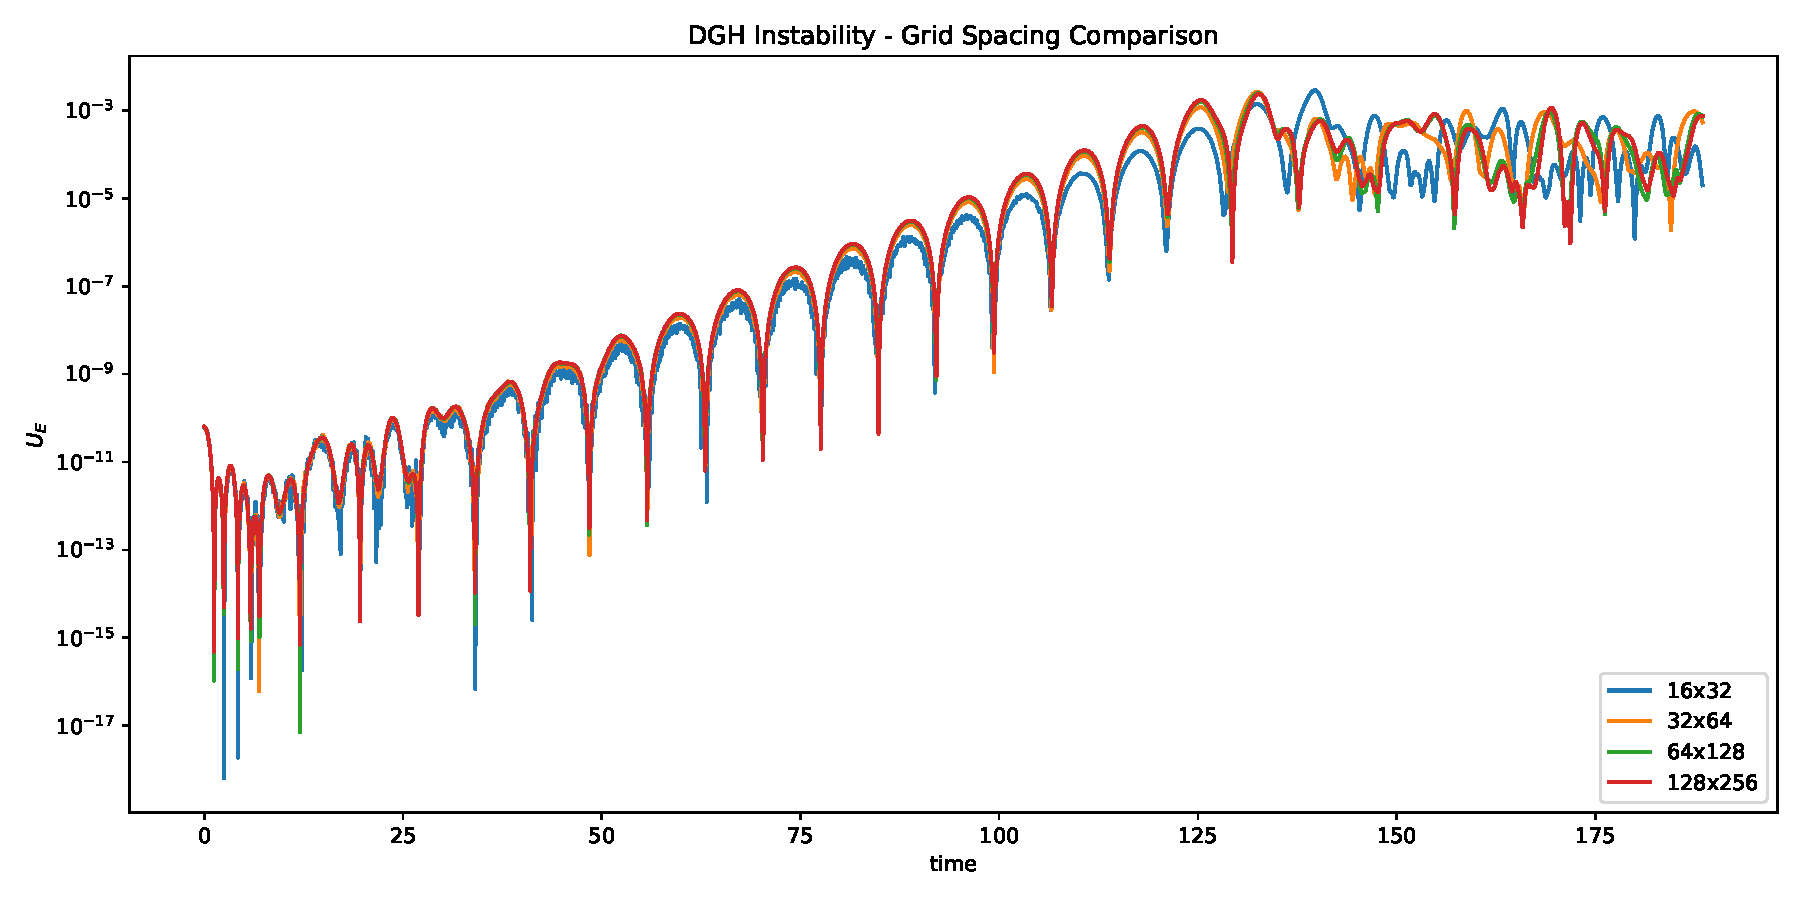
\includegraphics[width=0.9\linewidth]{proj4/dgh_grid_spacing_comparison.pdf}
\caption{\label{fig:dgh-grid-spacing-comparison}Simulation results for $\omega_p^2 / \omega_c ^2 = 10$ and $k v_\perp / \omega_c = 4.5$ with various grid resolutions. The grid resolution reported in the legend is $N_x x N_v$. The growth rates measured for each run in order of increasing resolution are $0.250$, $0.261$, $0.264$, $0.265$. The growth rate predicted by the linear theory is $0.265$.}
\end{figure}

\begin{table}[b]
\caption{\label{tab:frequency-values}Dominant wave mode observed in the PIC simulation of the initial ensemble shown in Figure \ref{fig:dgh-initial-distribution} for various values of $\mu \equiv k v_\perp / \omega_c$ with $\omega_p ^2 / \omega_c ^2 = 10$.}
\begin{ruledtabular}
\begin{tabular}{lrr}
$k v_\perp / \omega_c$&
$\text{Re}(\omega)$&
$\text{Im}(\omega)$\\
\colrule
4.1 & 1.30 & 0.190\\
4.5 & 1.39 & 0.265\\
5.0 & 1.6 & 0\\
5.6 & 2.38 & 0.296\\
6.0 & 2.46 & 0.202\\
6.6 & 4.09 & 0.192\\
\end{tabular}
\end{ruledtabular}
\end{table}

The ability of our PIC code to reproduce wave solutions is dependent on the grid spacing and the number of particles we use to sample the distribution function. To convince ourselves that we have made the grid sufficiently fine to capture the wave solutions of Eqn. \ref{fig:dgh-dispersion}, we can repeat the same analysis for a particular $\mu$ with a variety of grid resolutions. Since our PIC solver is second-order accurate in time and space, we expect to see second-order convergence to the predicted growth rate. As shown in Figure \ref{fig:dgh-grid-spacing-comparison}, the growth rate of the unstable mode converges to the valued predicted by linear theory.

\section{Conclusion}

Adding a static, uniform magnetic field to the electrostatic PIC code has allowed for the investigation of interesting phenomena only present in a uniformly magnetized plasma. The code is able to reproduce plasma waves perpendicular to the static, uniform magnetic field, to good agreement with the wave solutions predicted by a linear analysis of the Vlasov equation. The behavior predicted by the linear theory is replicated by the model, even with a very coarse grid spacing and relatively few particles. Increasing the grid resolution converges to the predicted growth rate, with second-order accuracy. The PIC model code is contained in the attached \texttt{pic1} Python module.

\nocite{*}

\bibliography{proj4}% Produces the bibliography via BibTeX.

\end{document}
